\documentclass[12pt]{article}
\usepackage[utf8]{inputenc}
\usepackage{fullpage}
\usepackage{graphicx}
\usepackage{hyperref}

\begin{document}

\section*{Throughput studies for data analysis applications}

\subsection*{Introduction}

High-speed data throughput is a requirement for most high energy physics software. Whether improving old software or developing new software, we must keep an eye on this aspect of its performance.

The metrics described in this section were measured as part of the development process for two new software products: root4j\footnote{\url{https://github.com/diana-hep/root4j}}, which provides access to ROOT files in Java (and therefore Apache Spark), and Femtocode\footnote{\url{https://github.com/diana-hep/femtocode}}, which is a query system, intended to produce plots from large (petabyte) datasets in real time.

Throughput bottlenecks can appear in three places. The first is loading into memory, which includes reading from physical disks and the network, deserialization, and decompression. The second is loading from memory into the processing unit, which is often much faster than the first and doesn't involve any transformations. The third is the computation itself. All three are relevant because caches may be employed to hide the effect of a slow load-into-memory or a slow load-from-memory.

For instance, root4j is called by spark-root\footnote{\url{https://github.com/diana-hep/spark-root}} to load data from ROOT files into Spark as a {\tt DataFrame}. After the first request (and until subsequent loads cause it to spill to disk), Spark caches the {\tt DataFrame}, distributing its contents across the random access memory of a whole cluster. Similarly, Femtocode is designed with the expectation that physicist users want to re-plot the same data several times in a row, tweaking aspects of the plot, so it also has a distributed, in-memory cache. In the first request, the disk or network bottleneck is relevant; afterward, the memory-to-processor bandwidth is relevant. The calculation itself may or may not overwhelm both of these, depending on what is being calculated. Simple histogram filling (the most common use-case for both Spark and Femtocode) requires much less processing time than load time.

We will therefore focus on the first two bottlenecks only: load-to-memory and memory-to-processor. Furthermore, each of these depend strongly on the hardware. Our software may be used on any hardware, so each of our metrics is a {\it comparison} of one software solution to another, both on the same hardware. These numbers should therefore be understood as relative, except where the specific hardware is described.

Code for all of these tests can be found in the {\tt diana-hep/femtocode-metrics} GitHub repository\footnote{\url{https://github.com/diana-hep/femtocode-metrics}}.

\subsection*{ROOT file reading: Java vs optimized C++}

The root4j library is a pure-Java implementation of ROOT file reading. This has technical advantages over alternatives that would call the standard C++ implementation of ROOT (JNI, UNIX pipes, or sockets): root4j is easy to install as a JAR from Maven Central and is free of several classes of bugs, including segmentation faults and failures in interprocess communication. It does, however, have the potential to be slower than the C++ implementation, since Java is a virtual machine with garbage collection.

Early in the development process, the read performance of root4j and C++ ROOT was compared to get a sense of this cost. Track $\chi^2$ values for all tracks (hundreds per event) were read from a CMS public dataset (AOD). This study focuses on a single attribute of a variable-length collection of objects within the event, so it relies heavily on the fact that these objects are laid out in a columnar fashion in the ROOT files.

Figure~\ref{root4j_reading_tracks} shows the reading rate as nanoseconds per track (left axis) and, equivalently, as megabytes per second for the {\it decompressed} data (right axis), measured every 100,000 tracks. Measuring this rate as a function of time is important because Java does HotSpot optimization at the beginning of the run, sacrificing start-up latency for long-term throughput.

\begin{figure}[t]
\begin{center}
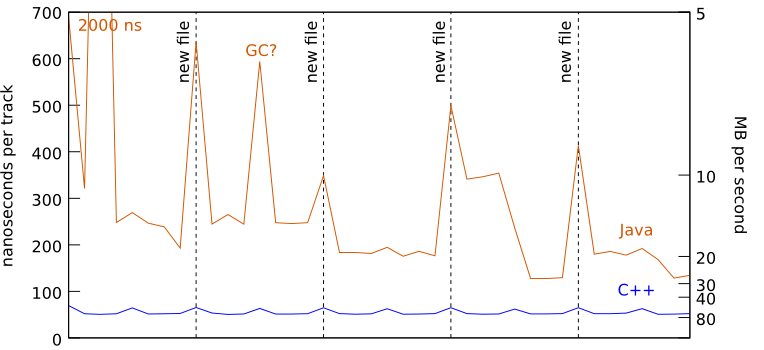
\includegraphics[width=0.8\linewidth]{root4j_reading_tracks.png}
\end{center}

\caption{\label{root4j_reading_tracks} Rate of reading track $\chi^2$ in root4j and C++ ROOT as a function of time. (Samples on the horizontal axis are every 100,000 tracks and ``MB'' refers to {\it decompressed} data.)}
\end{figure}

These files were also pre-read before measuring any data, so that they would be in Linux's memory cache, effectively removing the physical bottleneck of disk access and ensuring that neither software product is unfairly discounted because of this large bottleneck.

Both C++ and Java readers are deserializing and decompressing (deflate) the same bytes. The C++ ROOT version is 6.08/04 (pre-built binary for Ubuntu Linux). The root4j version is 0.1-pre2; spark-root and Spark were {\it not} involved in this test (which would complicate matters, due to caching). Both have been executed in a single process, single thread.

In the plot, we see that standard C++ ROOT is consistently faster than root4j. We also see that, unlike C++, root4j starts slow and accelerates. We see the HotSpot optimization phase as a spike (temporary slow-down) at the beginning of reading, a spike when opening each file, and a single spike in the middle of one file read. Spikes like these appear at different times in different runs, so they are likely garbage collector pauses.

However, the asymptotic speed of root4j, which is all that matters for large files and large datasets, is about four times slower than C++. Depending on the user's intended purpose, this cost may be worthwhile, since it opens direct access to all the ``big data'' and machine learning tools that have been developed for the Java platform.

More recent performance benchmarks are in development, using Spark's built-in performance counters\footnote{\href{https://github.com/diana-hep/spark-root/blob/master/md/PerformanceBenchmarksPublicDS.md}{\tt https://github.com/diana-hep/spark-root/blob/master/md/PerformanceBenchmarksPublicDS.md}}.

\subsection*{ROOT file reading: CMSSW vs optimized C++}

The second test of ROOT file reading was motivated by Femtocode, which takes advantage of ROOT's columnar data representation on disk to perform calculations in the same format in memory, without reconstructing objects. This is in contrast to a traditional framework for analyzing physics data, such as CMSSW.

CMSSW uses ROOT to build instances of C++ classes, and physicist users write C++ code to interact with those objects. Since arbitrary-length collections of record structures ({\tt std::vector<SomeClass>}) are common, these objects may not be contiguous in memory. Since the user code could access any attribute from these classes, all columns associated with the whole class must be loaded, even if the user actually accesses only one or two.

Femtocode, on the other hand, is a high level language that gets JIT-compiled to machine code. Part of this compilation process determines which attributes are needed and only loads those. The code is also compiled in such a way that it runs on contiguous arrays of data loaded directly from the ROOT file without constructing objects first.

Femtocode's strategy is similar to {\tt TTree::Draw}, a special-purpose function for aggregating data into histograms (and immediately drawing them). Femtocode and {\tt TTree::Draw} differ in that Femtocode is JIT-compiled and more general, but the similarities are close enough that a comparison to {\tt TTree::Draw} would be helpful.

Table~\ref{cmssw-table} compares the file-reading performance of CMSSW, {\tt TTree::Draw}, and a ROOT-reading routine designed for Femtocode. This specialized reader uses the ROOT libraries, but avoids function calls that would reconstruct C++ objects from the data, as an ordinary user would want. We thank Philippe Canal for his help in writing this routine.

\begin{table}[t]
\caption{\label{cmssw-table} File-reading rates in events per millisecond per process (kHz per process). In each case, the goal was only to access the $p_T$ (or $E_T$) attribute of each particle, though CMSSW loads all attributes associated with the particle.}

\begin{center}
\begin{tabular}{l c c c c c}
          &\# of particles & \# of attributes & CMSSW &{\tt TTree::} & Femtocode \\
particle  & per event (avg) & (``branches'') & EDAnalyzer &{\tt Draw()} & ROOT reader \\\hline
photon    & 2.9    & 205         & \mbox{\ \ \ \ \ } 1.14 kHz   &   \mbox{\ \ \ \ \ } 435 kHz       &   \mbox{\ \ \ \ \ } 769 kHz \\
electron  & 2.5     & 231         & 1.02   &   417       &   833        \\
muon      & 2.7     & 192         & 1.02   &   16.5      &   770        \\
tau       & 6.3     &  88         & 1.55   &   244       &   417        \\
jet       & 16.7    &  95         & 1.15   &   123       &   182        \\
AK8 jet   & 1.8     &  95         & 2.10   &   556       &   1000       \\
\end{tabular}
\end{center}
\end{table}

The CMSSW reader uses version {\tt 8\_0\_25} of the CMSSW software with a custom EDAnalyzer following current best-practices for file-reading ({\tt EDGetTokenT<>} and {\tt consumes<>} to inform CMSSW of which particles will be loaded). The goal was to extract the $p_T$ (or $E_T$) value from a variety of particles (individually, in separate runs). CMSSW is at a disadvantage for this kind of test because it must load all attributes of the selected particle because it doesn't analyze user code to see which are necessary. The different particle types have 95--231 attributes (called ``branches'' in ROOT), so for this task, CMSSW is reading a hundred times more data than necessary. This roughly correlates with its performance.

(Experiment frameworks like CMSSW were also designed for event reconstruction, which requires many more attributes per particle and has a performance that is closer to optimal.)

The {\tt TTree::Draw} function was designed to plot small numbers of branches, so it does not load unnecessary attributes. Similarly, Femtocode is primarily intended for plotting, so its specialized reader calls a similar set of functions as {\tt TTree::Draw}. In most cases, their results are within a factor of 2 of each other, though the muon comparison is a factor of 50. (This has been reported to the ROOT team; they are investigating.) The factor of 2 can be expected, since {\tt TTree::Draw} is additionally invoking an interpreter to generate a plot, unlike the other readers, which simply add up $p_T$ values (to ensure that it is not eliminated by the compiler).

All tests were single-process, single-thread, reading the same input file that was pre-loaded into Linux cache by previous reads. The {\tt TTree::Draw} tests were rotated in order and the first call was discarded, since {\tt TTree::Draw} does some initialization the first time it is called.

In addition to comparing these three ways of calling ROOT routines to read ROOT files, we tested the time required to read a flat array of the same size from a Numpy file. Numpy files have a very simple format: the contiguous array is compressed (deflate, same as ROOT) and written to disk as-is (with a small header). The Femtocode ROOT reader was only 5\% slower than reading the equivalent data from Numpy files, which suggests that the procedure is near optimal.

\subsection*{Memory bandwidth: conventional vs GPU vs KNL}

Because of the high cost of loading data into memory, Spark and Femtocode cache that data for subsequent computations. This fits the work-pattern of data analysis, in which a computation is often repeated with subtle variations as part of exploratory data analysis or systematics studies. Assuming that the whole dataset can be loaded, all but the first pass benefit from the cache, often by orders of magnitude (100--1000$\times$).

At these high rates, the bottleneck shifts from disk or network to the DRAM memory. For a sample plotting problem, we performed a simple operation (addition) on 10 billion double-precision floating point numbers. We arrived at this figure because 100 million events is typical of a high energy physics dataset (all $t\bar{t}$ data collected by CMS since its inception is 100~fb$^{-1}$ $\times$ 1~nb = 100 million events) and the plotting code may need to access 100 values per event (hundreds of tracks or combinations of attributes). This is 80~GB of in-memory data to be evaluated while the user waits.

The throughput from DRAM to CPU back to DRAM is highly affected by compiler optimizations, which target this specific problem. In a single process, single thread, the following times are required to either add values to the array in-place or add them and store them elsewhere (``immutable'' operation):

\begin{center}
\begin{tabular}{r | c c c c}
           & with {\tt -O0} & with {\tt -O1} & with {\tt -O2} & with {\tt -O3} \\\hline
in-place   & 87.8~sec       & 27.2           & 27.1           & 25.6~sec       \\
immutable  & 91.2~sec       & 38.7           & 39.2           & 39.2~sec       \\
\end{tabular}
\end{center}

Without compiler optimizations, the in-place and immutable times are nearly the same, even though the first accesses one memory location and the second accesses two. With optimizations, both operations are faster, but the one with fewer memory accesses is more so. These optimizations involve such things as loop unrolling, which hide the latency of reading from memory. Automatic vectorization, which is a potential optimization unrelated to memory access, is only applied in {\tt -O3}, and we don't see the effect here.

Plotting problems are embarrassingly parallel and can be horizontally scaled to a nearly arbitrary degree, dividing this 25 or 40~seconds by a large factor of $N$. However, we also wanted to see if specialized hardware could solve the problem. We performed the same simple operation on several different GPUs and one Knight's Landing (KNL) chip.

The GPU results are summarized in Table~\ref{gpu-results}. For comparison, the single-threaded CPU rates are 0.39~GHz (in-place) and 0.26~GHz (immutable): fully vectorized GPU rates range from 4.0~GHz to 56.9~GHz for laptop/gaming GPUs (GeForce GTX) to high-end supercomputing GPUs (Tesla P100).

\begin{table}[t]
\caption{\label{gpu-results} Data throughput rates in GHz (billions of 32-bit floating point values per second) for various GPUs and architectures. The first line is a data copy that does not involve the GPU, for comparison with the ones that do. ``Unified'' memory (also known as ``pinned'') are pointers that can be accessed by both host (CPU) and device (GPU), but with a price in performance, as we see below. ``Global'' memory is bound to the GPU and requires an explicit copy.}

\begin{center}
\begin{tabular}{l c c c c c c}
                  &  GeForce & GRID     & Tesla       & Tesla  & Tesla  & Tesla     \\
                  &  GTX     & K520     & K20m        & K40c   & K20Xm  & P100-SXM2 \\
                  &  660M    & (AWS)    & (Princeton) & (CERN) & (CERN) & (CERN)    \\
\underline{Data transfers:}   &          &          &             &        &        &           \\
DRAM to {\it CPU} & 1.8      & 1.5      & 0.82        & 0.77   & 0.77   & 3.5       \\       
                  &          &          &             &        &        &           \\
DRAM to GPU       & 1.7      & 1.0      & 0.87        & 0.82   & 0.51   & 3.4       \\  
GPU to DRAM       & 1.7      & 1.0      & 0.51        & 0.49   & 0.76   & 1.8       \\ 
CPU write unified & 2.3      & 1.5      & 0.87        & 0.82   & 0.50   & 3.6       \\      
CPU read unified  & 2.3      & 1.5      & 0.50        & 0.48   & 0.46   & 2.1       \\     
within GPU        & 7.0      & 15.2     & 18.9        & 23.6   & 23.6   & 56.9      \\      
                  &          &          &             &        &        &           \\
\underline{Calculations:}     &          &          &             &        &        &           \\
in-place global   & 4.0      & 13.7     & 16.9        & 21.4   & 21.1   & 56.9      \\
immutable global  & 4.1      & 14.3     & 16.9        & 21.5   & 21.2   & 56.9      \\ 
in-place unified  & 2.6      & 2.2      & 1.4         & 2.6    & 1.6    & 7.1       \\
immutable unified & 2.9      & 2.4      & 1.5         & 2.9    & 2.9    & 8.3       \\
\end{tabular}
\end{center}
\end{table}

%% milliseconds for 1 GB, but times (ms) are underestimated by a factor of 8
%% DRAM to {\it CPU} & 18.6     &    21.71 &       40.96 &  43.43 &  43.40 &      9.71 \\
%% DRAM to GPU       & 19.8     &    34.56 &       38.68 &  41.11 &  66.12 &      9.92 \\
%% GPU to DRAM       & 19.8     &    34.07 &       65.27 &  68.24 &  44.17 &     18.18 \\
%% CPU write unified & 14.5     &    21.87 &       38.49 &  40.95 &  67.66 &      9.41 \\
%% CPU read unified  & 14.5     &    22.36 &       67.34 &  70.27 &  72.30 &     16.33 \\
%% within GPU        &  4.8     &     2.21 &        1.78 &   1.42 &   1.42 &      0.59 \\
%%                   &          &          &             &        &        &           \\
%% Calculations:     &          &          &             &        &        &           \\\hline
%% in-place global   &  8.4     &     2.45 &        1.99 &   1.57 &   1.59 &      0.59 \\
%% immutable global  &  8.1     &     2.35 &        1.98 &   1.56 &   1.58 &      0.59 \\
%% in-place unified  & 12.8     &    15.09 &       23.37 &  13.02 &  20.75 &      4.73 \\
%% immutable unified & 11.5     &    14.02 &       21.72 &  11.42 &  11.65 &      4.03 \\

%% awk '{print 1e-9/(8*$1/1000/1024/1024/1024*4), 1e-9/(8*$2/1000/1024/1024/1024*4), 1e-9/(8*$3/1000/1024/1024/1024*4), 1e-9/(8*$4/1000/1024/1024/1024*4), 1e-9/(8*$5/1000/1024/1024/1024*4), 1e-9/(8*$6/1000/1024/1024/1024*4)}'

Another thing to notice is that memory-to-CPU and memory-to-GPU bandwidths are similar to each other for most architectures: the biggest deviation is 60\% slower for copying to the GPU. In designing software, we can consider the GPU to be just as ``distant'' from memory as the CPU.

Once the data are on the GPU (as ``global'' memory, not ``unified''), calculations are much faster. In particular, copying data within the GPU has approximately the same cost as a calculation. The following hierarchy emerges:
\begin{center}
DRAM to CPU $\sim$ to GPU $\ll$ GPU global memory to calculation $\sim$ to copy.
\end{center}
For designing software, this (a) that there's no memory bandwidth advantage to performing operations in-place, rather than immutably, and (b) that the GPU is advantageous only if several operations can be performed before copying the data back to normal memory. We may even consider keeping an input data cache in GPU global memory as well as DRAM.

Finally, it's worth pointing out that the ``unified'' memory model provided by modern CUDA hides the cost of the transfer. In the unified model, host (CPU) code and device (GPU) code use the same pointers without an explicit copy, but GPU calculations on unified memory run at a much lower rate than explicit global memory. Presumably, it is copying on demand.

(GPU ``shared'' memory is faster than global, but much too small for our datasets.)

Finally, this comparision of single-threaded CPU rates (0.26~GHz) to GPU rates (4--57~GHz) is unfair because modern architectures support multiple CPU cores, often many more (8--64) than the number of GPUs (1--4).

Given the embarrassingly parallel nature of the problem, we would naively expect perfect scaling with the number of worker threads up to the number of cores. On conventional and even NUMA architectures, however, we find a limit of about 2~GHz. Since these processes do not interact, we conjectured that the limiting factor was contention on the memory bus, since all workers are doing little more than requesting data. Even in NUMA architectures, half of the CPUs share a single memory bus.

To prove this conjecture, we obtained access to a Knight's Landing (KNL) architecture at Princeton. KNL has one feature in common with GPUs: small groups of CPU cores have a local pool of memory called MCDRAM, which is a rough equivalent of a GPU's global memory (in size, granularity, and distance from the processing unit). If the 2~GHz scaling limit is due to memory bus contention, moving data to a KNL's MCDRAM would reduce that contention and allow higher scaling.

Figure~\ref{knl-scaling} shows that the conjecture was right: switching from a conventional architecture to KNL does not, by itself, break the 2~GHz limit, but allocating memory on the MCDRAM does. In fact, scaling on a single KNL machine reaches 8~GHz with 128 cores, twice the number of physical cores (though it drops precipitously beyond that).

\begin{figure}[t]
\begin{center}
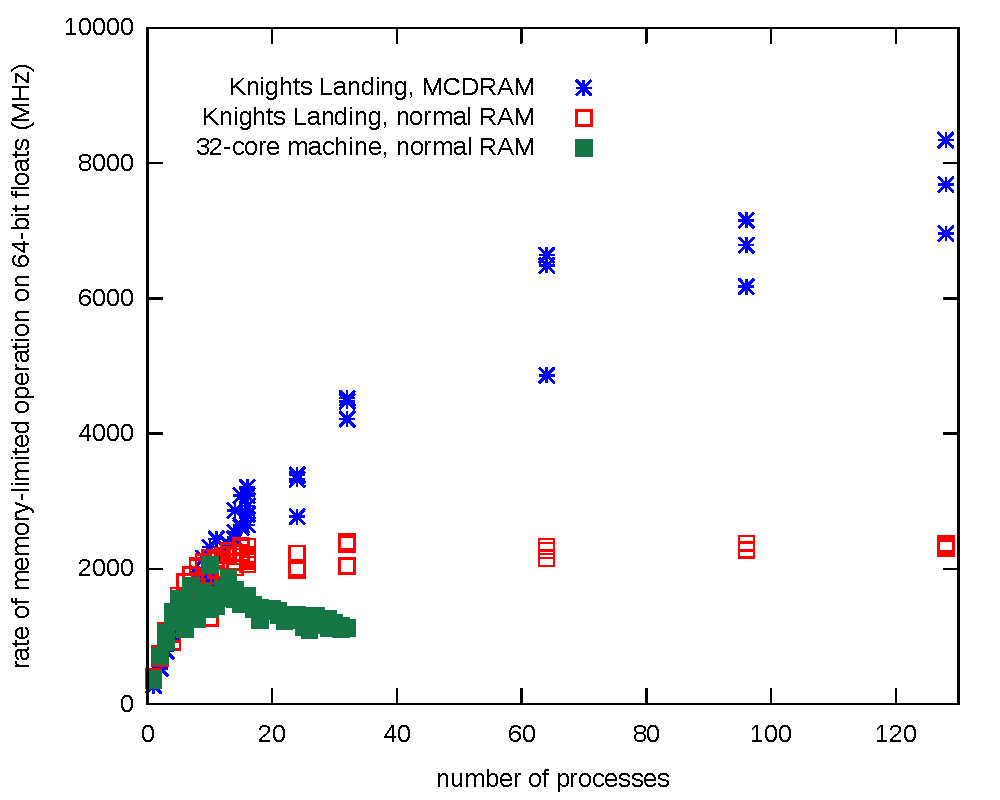
\includegraphics[width=0.8\linewidth]{knl-scaling.pdf}
\end{center}

\caption{\label{knl-scaling} Memory bandwidth-limited scaling on a conventional 32-core machine, a Knight's Landing machine with input data in globally shared DRAM and local MCDRAM, respectively.}
\end{figure}

All of these studies point to the same general conclusion, that novel hardware like GPUs and KNL are advantageous for our project not because of superior computational ability but because they have local stores of memory, close to the computing elements. Our gains in throughput exclusively depend on how well we exploit the device memory.

While the computational problem Femtocode poses is embarrassingly parallel, not all parts of it are vectorizable. To perform the equivalent of object oriented programming on data represented as flat arrays, some operations need to correlate values in arrays of different lengths. These operations, known in Femtocode as ``explode'' and ``combine'', are not a good match to the GPU's vectorized programming model. Explode operations must interpret an array sequentially from start to end, and combine operations must either be sequential or require $\log_2 N$ vectorized passes over a dataset of $N$ elements. These operations are best suited for a sequential processor like KNL or a conventional CPU, with GPUs used only for the ``flat'' operations that correlate equal-length arrays element by element.

Finally, memory bus contention can also be defeated by purchasing a larger number of fewer-core machines. This is another way to make memory more local: by physically separating them on the rack. It is an open question how the price of four 16-core servers compares to the price of one 64-core KNL, for instance. However, this question is not a blocker for writing software.

\subsection*{Conclusions}

In this section, we described several quantitative analyses we performed as part of designing software for data analysis applications. We confirmed the disk $\ll$ memory $\ll$ processing hierarchy, with some useful details.

C++ ROOT remains the fastest way to read ROOT files, though it depends on how this library is used. In our application of extracting only one or a few attributes of each particle for plotting, we can pull data from the file at a rate of about a MHz per thread. Java is four times slower, but it brings the benefit of providing access to Big Data and machine learning tools like Apache Spark.

Using (one might say ``misusing'') an experiment's framework like CMSSW for the purpose of extracting only one attribute per particle is three orders of magnitude slower: about a kHz. This is primarily because CMSSW loads all attributes per particle (they are needed for the usual application of event reconstruction) but partly because CMSSW creates and destroys C++ objects in non-contiguous memory for the convenience of the user.

The MHz rate of {\tt TTree::Draw} and the Femtocode ROOT reader is nearly identical to the rate of reading numbers from a Numpy file, which has minimal overhead. Therefore, this MHz rate is probably close to the maximum possible.

If the input data are in a memory cache, however, rates of a quarter GHz per thread are possible (almost three orders of magnitude faster). Adding non-interacting threads allows us to scale up to 2~GHz before running into memory bandwidth limits of a conventional memory bus. However, using local memory attached to a KNL or GPU device breaks through this limit, allowing up to 8~GHz on a KNL and 57~GHz on a high-end GPU.

Amusingly, these event-processing rates even exceed the collision rate in the LHC, though the similarity is coincidental. Collision events are highly filtered, and we need a system to process years of collected data in seconds if it is to serve for real-time analysis.

\end{document}
